\documentclass[conf]{new-aiaa}

% --- PACKAGES ---
\usepackage{amsmath}
\let\Bbbk\relax % Resolve conflict with newtxmath
\usepackage{amssymb}
\usepackage{booktabs}
\usepackage{graphicx}
\usepackage{url}
\usepackage{algorithm}
\usepackage{algpseudocode}
% \usepackage{cite} % AIAA template uses natbib via new-aiaa class
\usepackage{authblk}

% --- GRAPHICS PATH ---
\graphicspath{{figures/}}

% --- TIKZ & GRAPHICS SETUP ---
\usepackage{tikz}
\usetikzlibrary{arrows.meta, positioning, shapes.geometric, calc, backgrounds, fit}

% --- COLOR DEFINITIONS (User Specified) ---
\definecolor{Garnet}{HTML}{73000A}
\definecolor{CSecondaryRed}{HTML}{CC2E40}
\definecolor{CBlue}{HTML}{466A9F}
\definecolor{CDark}{HTML}{1F414D}
\definecolor{COlive}{HTML}{65780B}
\definecolor{CLime}{HTML}{CED318}
\definecolor{CGold}{HTML}{A49137}
\definecolor{CGrayLight}{HTML}{E5E5E5}
\definecolor{CGrayDark}{HTML}{555555}

% --- TIKZ STYLES ---
\tikzset{
    flatblock/.style={
        rectangle,
        draw=black,
        fill=white,
        text width=2.8cm,
        minimum height=1.2cm,
        align=center,
        font=\footnotesize\sffamily,
        line width=0.8pt
    },
    data/.style={
        rectangle,
        draw=Garnet,
        fill=Garnet!5,
        text width=2.8cm,
        minimum height=1.2cm,
        align=center,
        font=\footnotesize\sffamily,
        line width=0.8pt
    },
    decision/.style={
        diamond,
        aspect=2,
        draw=CBlue,
        fill=CBlue!5,
        text width=2.0cm,
        align=center,
        font=\scriptsize\sffamily,
        line width=0.8pt
    },
    flatarrow/.style={
        ->,
        >={Latex[length=3mm, width=2mm]},
        draw=CDark,
        line width=1.0pt
    },
    labeltext/.style={
        font=\scriptsize\sffamily,
        color=CDark
    }
}

\title{Dual-Camera Active Acquisition for Automated Small-Object Dataset Construction}

\author{Jackie Wang\footnote{Graduate Student, Department of Mechanical Engineering, AIAA Student Member.}}
\author{JC Vaught\footnote{Graduate Student, Department of Mechanical Engineering, AIAA Student Member.}}
\author{Douglas Cahl\footnote{Professor, Department of Mechanical Engineering.}}
\author{Yi Wang\footnote{Professor, Department of Mechanical Engineering.}}

\affil{Department of Mechanical Engineering, University of South Carolina, Columbia, SC, 29201}

\begin{document}

\maketitle

\begin{abstract}
Deep learning performance on small objects is frequently bottlenecked by the quality and quantity of training data rather than model architecture. To address this, we propose an active dual-camera system for automated small-object dataset generation, specifically designed to overcome the resolution limits of static wide-angle surveillance. The system leverages a fixed wide-angle camera for target discovery and a PTZ unit for detailed interrogation. The control framework transitions from open-loop predictive slewing to closed-loop visual tracking, compensating for mechanical latencies and slow zoom mechanics. Implemented on an NVIDIA Jetson Orin, the system runs concurrent detector instances, one on the GPU and one on the Deep Learning Accelerator (DLA) to achieve 30 fps throughput. High-resolution object verifications are projected back into the wide frame using a static homography-based calibration, creating high-confidence labels for targets that appear as only a few pixels in the wide view. We validate the system design against a test case of distant aircraft in daylight, analyzing the trade-offs between slew speed ($120^\circ$/s) and zoom settling time. Preliminary analysis suggests this active acquisition paradigm can improve label precision significantly and reduce the human effort required for small-object dataset curation.
\end{abstract}

\section{Introduction}
While recent surveys \cite{chen2020survey, nikouei2024smallobj} have demonstrated significant architectural improvements in generic object detection, they have failed to fully solve a problem that has persisted for decades: small object detection. The core issue remains one of pixel-level information loss, since no amount of digital zoom can recover details that were never sampled. Although some super-resolution algorithms show promise by recovering detail via temporal information, these methods are often computationally intensive and ill-suited for strict real-time inference \cite{mahaur2022superres}.
\par
Even with high-resolution imagery, real-time detection pipelines typically downsample inputs to manageable resolutions (e.g., $640 \times 640$) to satisfy compute constraints. This reduction inherently compresses distant targets into featureless blobs that are difficult to classify without relying on temporal context (as humans do) or additional sensor modalities \cite{rozantsev2017flying}.
\par
In the case of distant aerial surveillance, a target may occupy fewer than $15 \times 15$ pixels in a wide-angle feed. At this resolution, distractors (i.e. birds, cloud edges, specular highlights, or sensor noise) are indistinguishable from the target of interest. Standard digital zooming (cropping) only magnifies these ambiguities \cite{zhang2019zoom}. To achieve robust detection, a dataset must contain examples where these confusing cases are resolved, yet human labelers often cannot distinguish them in raw wide-angle footage.
\par
We address this by replacing the human labeler with a dual-camera system designed to automate the construction of small-object datasets. A fixed wide-angle camera provides persistent coverage, while a controllable Pan-Tilt-Zoom (PTZ) camera provides resolution on demand. The key technical challenge lies in the handover, since the system must move a mechanical lens to capture a moving target based on delayed visual data. This system compensates for the $\approx 150$\,ms latency between sensor capture and motor response and achieves high movement rates ($120^\circ$/s) without inducing motion blur.
\par
The contributions of this work are presented as follows: i) a hardware-software architecture that synchronizes wide-angle search with narrow-angle verification; ii) a predictive control formulation that compensates for system latency to enable reliable active target acquisition from wide-angle cues; and iii) a validated pipeline for label transfer, showing how distracting objects rejected by the PTZ can be automatically added to the wide-angle dataset to reduce false positives in future deployment.

\section{Related Work}
\subsection{Small Object Detection}
Recent surveys synthesize methods for small object detection, highlighting multi-scale feature processing, super-resolution or enhancement, context modeling, and data-centric strategies such as targeted acquisition and hard-negative mining.
\par
For airborne targets, YOLO-family detectors are commonly chosen for their speed--accuracy trade-off, and recent work explicitly evaluates YOLOv8-based pipelines for flying object detection.

\subsection{PTZ Tracking and Active Vision}
PTZ tracking differs from fixed-camera tracking because the camera motion changes the image formation process and induces highly dynamic backgrounds. Standardized evaluation of PTZ trackers and benchmark methodologies have been studied, emphasizing control latency, re-centering accuracy, and zoom stability.
\par
Modern active vision approaches incorporate deep detection modules into PTZ decision-making for improved observation quality, including PTZ-assisted perception pipelines and PTZ-guided small-object detection strategies.
\par
For small aerial targets, recent systems explicitly coordinate wide sensing with PTZ imaging and tracking to keep fast, erratically moving targets in view.

\subsection{Pseudo-Labeling, Self-Training, and Active Learning}
Pseudo-labeling and self-training reduce annotation costs by selecting high-confidence predictions as training targets, but they require careful thresholding and quality control to avoid drift. Adaptive thresholding strategies for pseudo-label selection have been proposed to reduce manual tuning, and recent object detection self-training methods emphasize robust selection mechanisms.
\par
Active learning for object detection studies how uncertainty and diversity can guide sample selection for labeling, including plug-and-play strategies that combine uncertainty- and diversity-based phases.
\par
This paper differs in that the ``labeling oracle'' is not a human annotator but a sensor action: the PTZ zoom. The acquisition action produces a higher-fidelity view that improves label quality and reduces ambiguity without manual annotation.

\section{System Overview}
\subsection{Hardware and Software Roles}
The system uses two cameras mounted with a fixed relative pose (Fig.~\ref{fig:hardware}):
\par
(1) a fixed wide-angle camera providing continuous coverage and running a real-time YOLO-family detector; \par
(2) a PTZ camera whose pan, tilt, and zoom can be commanded via a control interface and whose telemetry is logged with timestamps.
\par
The wide camera produces candidate detections and tracklets. A scheduling policy selects targets and commands the PTZ to re-center and zoom. The PTZ stream is analyzed to confirm class and refine bounding boxes. High-confidence PTZ detections are transferred back to the wide-angle frame to create dataset labels. A curation module filters low-quality frames and controls redundancy.

\begin{figure}[t]
\centering
\includegraphics[width=1.0\columnwidth]{fig_cameras_side_by_side.pdf}
\caption{Physical hardware configuration. A fixed wide-angle camera provides persistent coverage while a 2-axis PTZ camera can be commanded to lock onto and zoom in on candidate targets.}
\label{fig:hardware}
\end{figure}

\begin{figure}[t]
\centering
\includegraphics[width=0.75\columnwidth]{fig_fov_understanding_topdown.pdf}
\caption{Field of view comparison. The wide camera (blue) covers approximately $90^\circ$ for persistent surveillance, while the PTZ camera (red) provides a narrow, steerable, high-resolution view that can be directed to any point within the wide FOV.}
\label{fig:fov}
\end{figure}

\subsection{End-to-End Pipeline Diagram}
\begin{figure}[t]
\centering
\includegraphics[width=\columnwidth]{fig_pipeline.pdf}
\caption{Dual-camera active acquisition loop. The PTZ camera is triggered by wide-angle detections to improve evidence quality; high-confidence PTZ detections are transferred back to wide-angle frames.}
\label{fig:pipeline}
\end{figure}



\section{Problem Formulation}
Let $I^w_t$ be the wide-angle frame at time $t$, and let $I^p_t$ be the PTZ frame captured at time $t$ with telemetry $\tau_t = (\theta_t,\phi_t,z_t)$ representing pan, tilt, and zoom. The wide detector produces candidate detections $D_t = \{(b^w_{t,i}, s^w_{t,i}, c_{t,i})\}_i$ with bounding boxes $b^w_{t,i}$, confidence scores $s^w_{t,i}$, and class labels $c_{t,i}$.
\par
The system chooses actions $a_t$ that either keep scanning (no PTZ) or command the PTZ to acquire a zoomed observation centered on a selected candidate. The goal is to maximize the expected dataset value subject to control and compute constraints:
\begin{equation}
\max_{\pi} \ \mathbb{E}\left[\sum_t U\left(I^w_t, I^p_t, \tau_t\right)\right]
\end{equation}
subject to PTZ dynamics, latency, bandwidth, and storage budgets.
Here $U(\cdot)$ is an acquisition utility that increases with (i) label correctness probability, (ii) localization quality, (iii) novelty/diversity, and (iv) usefulness for training (hard examples and hard negatives).

\section{Calibration and Cross-View Geometry}
\subsection{Camera Model}
Both cameras are modeled with intrinsics $(K_w, K_p)$ and distortion parameters. Let $\Pi(\cdot)$ be perspective projection with distortion, and let $R_{pw}, t_{pw}$ map 3D points from wide-camera coordinates to PTZ-camera coordinates.
\par
For sky targets at long range, parallax between cameras is often negligible if the baseline is small relative to range. In that regime, direction-only transfer is effective: rays from each camera correspond to the same world direction, and cross-view mapping can be performed using ray directions on the unit sphere rather than estimated depth.


\subsection{Mapping Wide Detections to PTZ Pan/Tilt Commands}
Let $(u,v)$ be the center of a wide detection box $b^w$ in pixel coordinates. After undistortion, the bearing direction in the wide camera frame is
\begin{equation}
\hat{d}_w = \frac{K_w^{-1}[u \ v \ 1]^\top}{\|K_w^{-1}[u \ v \ 1]^\top\|}.
\end{equation}
Transforming to the PTZ base frame gives $\hat{d}_p = R_{pw}\hat{d}_w$. Using a conventional yaw--pitch parameterization, the commanded pan (yaw) and tilt (pitch) are
\begin{equation}
\theta = \mathrm{atan2}(\hat{d}_{p,y}, \hat{d}_{p,x}), \quad
\phi = \mathrm{atan2}(\hat{d}_{p,z}, \sqrt{\hat{d}_{p,x}^2+\hat{d}_{p,y}^2}).
\end{equation}
Because PTZ motion and video pipelines have latency, $\hat{d}_p$ is preferably computed from a short-horizon prediction of target motion rather than the instantaneous detection center.

\subsection{Zoom Selection by Target Angular Size}
Let $h^w$ be the detected box height in wide pixels. Under small-angle approximation, the apparent angular height is approximately $\alpha \approx h^w / f_w$, where $f_w$ is the wide focal length in pixels. To obtain a desired PTZ pixel height $h^p_{\mathrm{des}}$, select a PTZ focal length $f_p(z)$ such that
\begin{equation}
h^p_{\mathrm{des}} \approx \alpha f_p(z) \approx \frac{h^w}{f_w} f_p(z),
\end{equation}
then choose the zoom $z$ whose calibrated $f_p(z)$ best matches the required value, clipped to PTZ limits. This approach avoids explicit range estimation and is well suited for distant aircraft.


\section{PTZ Triggering, Tracking, and Scheduling}
PTZ tracking is a coupled perception-and-control problem with dynamic imaging conditions and control delays. Prior PTZ tracking evaluations emphasize that camera motion, latency, and re-centering quality dominate performance differences in practice.
\par
We use wide-camera tracklets to provide temporal coherence and to predict target bearing during PTZ motion. A lightweight predictor (e.g., constant angular velocity with $\alpha$--$\beta$ filtering or a Kalman filter) provides a predicted bearing $\hat{d}_w(t+\Delta)$ given command latency $\Delta$, consistent with classical pan/tilt tracking formulations.

\begin{figure}[t]
\centering
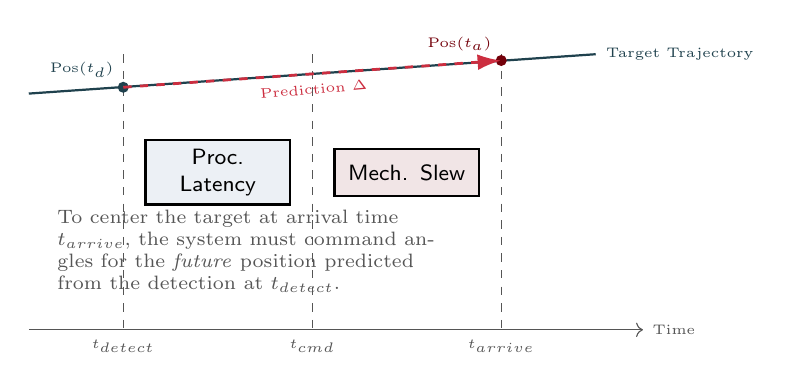
\begin{tikzpicture}[x=1.2cm, y=1.0cm]
    % Axes
    \draw[->, CGrayDark] (0,0) -- (6.5,0) node[right, font=\tiny] {Time};

    % Events on timeline
    \draw[dashed, CGrayDark] (1, 3.5) -- (1, 0) node[below, font=\tiny] {$t_{detect}$};
    \draw[dashed, CGrayDark] (3, 3.5) -- (3, 0) node[below, font=\tiny] {$t_{cmd}$};
    \draw[dashed, CGrayDark] (5, 3.5) -- (5, 0) node[below, font=\tiny] {$t_{arrive}$};

    % Target Motion Path (Top)
    \draw[thick, CDark] (0,3) -- (6, 3.5) node[right, font=\tiny] {Target Trajectory};
    \fill[CDark] (1, 3.08) circle (2pt) node[above left, font=\tiny] {Pos($t_d$)};
    \fill[Garnet] (5, 3.42) circle (2pt) node[above left, font=\tiny] {Pos($t_a$)};

    % Latency Blocks
    \node[flatblock, fill=CBlue!10, text width=1.6cm, minimum height=0.6cm] at (2, 2) {Proc. Latency};
    \node[flatblock, fill=Garnet!10, text width=1.6cm, minimum height=0.6cm] at (4, 2) {Mech. Slew};

    % Prediction Arrow
    \draw[flatarrow, color=CSecondaryRed, dashed] (1, 3.08) -- node[below, rotate=5, font=\tiny, color=CSecondaryRed] {Prediction $\Delta$} (5, 3.42);

    % Explanation Text
    \node[anchor=west, text width=5cm, font=\scriptsize, color=CGrayDark] at (0.2, 1.0) {
        To center the target at arrival time $t_{arrive}$, the system must command angles for the \textit{future} position predicted from the detection at $t_{detect}$.
    };
\end{tikzpicture}
\caption{Latency Compensation. The PTZ command must account for processing delays and mechanical slew time. The target position is extrapolated $\Delta$ seconds into the future to ensure the PTZ arrives at the correct bearing.}
\label{fig:latency}
\end{figure}

\begin{algorithm}[t]
\caption{Real-time wide-to-PTZ acquisition}
\begin{algorithmic}[1]
\State Init $f_{\theta}$ (wide), $\mathcal{T}$ (tracker), $g$ (PTZ), $\mathcal{D}$ (data)
\For{each wide frame $I^w_t$}
\State $D_t \leftarrow f_{\theta}(I^w_t)$; \quad $\mathcal{T}\leftarrow \mathrm{UpdateTracks}(\mathcal{T}, D_t)$
\State Compute $U(o)$ for tracks (conf, size, novelty)
\State Select $o^\star \leftarrow \arg\max U(o)$ s.t. availability
\If{$U(o^\star)>\tau_{\mathrm{trigger}}$}
\State Predict $\hat{d}_w(t+\Delta)$; map to $(\theta,\phi, z)$
\State Command PTZ: $g(\theta,\phi,z)$; get $I^p_{t'}$, $\tau_{t'}$
\State Run PTZ detector: $D^p_{t'} \leftarrow f_{\theta_p}(I^p_{t'})$
\If{Quality OK AND $\max s^p > \tau_{\mathrm{confirm}}$}
\State $b^{w\leftarrow p} \leftarrow \mathrm{Project}(b^p,\tau_{t'})$
\State Commit $(I^w_t, b^{w\leftarrow p}, c)$ to $\mathcal{D}$
\EndIf
\EndIf
\EndFor
\State Periodically retrain $f_{\theta}$ on $\mathcal{D}$
\end{algorithmic}
\end{algorithm}

\subsection{Utility Function for Triggering and Redundancy Control}
The trigger utility balances value and cost. A practical form is a weighted sum of terms:
\begin{equation}
U(o) = \lambda_1\,\mathrm{Unc} + \lambda_2\,\mathrm{SizeGain} + \lambda_3\,\mathrm{Novelty} - \lambda_4\,\mathrm{Cost},
\end{equation}
where $\mathrm{Unc}$ increases when the wide detector is unsure (so PTZ confirmation is valuable), $\mathrm{SizeGain}$ estimates how much the PTZ will increase target pixels, $\mathrm{Novelty}$ reduces redundancy by down-weighting near-duplicates, and $\mathrm{Cost}$ captures PTZ time-on-target, slew distance, and opportunity cost (only one PTZ target at a time).
\par
This framing is consistent with object-detection active learning literature that combines uncertainty and diversity, although here the action is a sensor query rather than a human label request.

\section{Automated Dataset Construction}
\subsection{Label Sources and Cross-View Transfer}
The PTZ view is treated as a higher-fidelity label source when it produces a confirmed detection for the target class. The label transfer module maps the PTZ detection back into the wide image coordinate system.
\par
For distant targets, direction-only transfer proceeds by converting the PTZ bounding box corners into bearing rays, rotating those rays into the wide camera frame, and projecting them into the wide image plane. Let $(u^p_k,v^p_k)$ be PTZ box corners; compute PTZ rays $\hat{d}^p_k$ from $K_p^{-1}$, rotate to wide frame $\hat{d}^w_k = R_{wp}\hat{d}^p_k$, then project:
\begin{equation}
[u^w_k, v^w_k, 1]^\top \propto K_w \hat{d}^w_k, \quad k \in \{1,2,3,4\}.
\end{equation}
The transferred wide box is the tight axis-aligned rectangle enclosing the projected corners. This procedure uses only calibrated intrinsics and the relative rotation, plus the PTZ telemetry that defines the effective PTZ optical axis at capture time.

\subsection{Quality Gates and Drift Prevention}
Self-training and pseudo-labeling can suffer from confirmation bias if low-quality pseudo-labels are admitted. This is widely recognized in semi-supervised detection; adaptive thresholding and robust pseudo-label selection reduce manual tuning and improve stability.
\par
In this system, the primary drift control mechanism is the physical zoom verification: many ambiguous wide detections become unambiguous at higher resolution. Remaining failure modes are handled by quality gates (Fig.~\ref{fig:gates}) that reject samples when motion blur is excessive, exposure is saturated (e.g., sun glare), the target is at the frame boundary, or the PTZ detector disagrees with the wide detector class in a way indicative of confusion (e.g., airplane vs bird). Each gate is implemented as a deterministic predicate so that dataset inclusion is reproducible and auditable.

\begin{figure}[t]
\centering
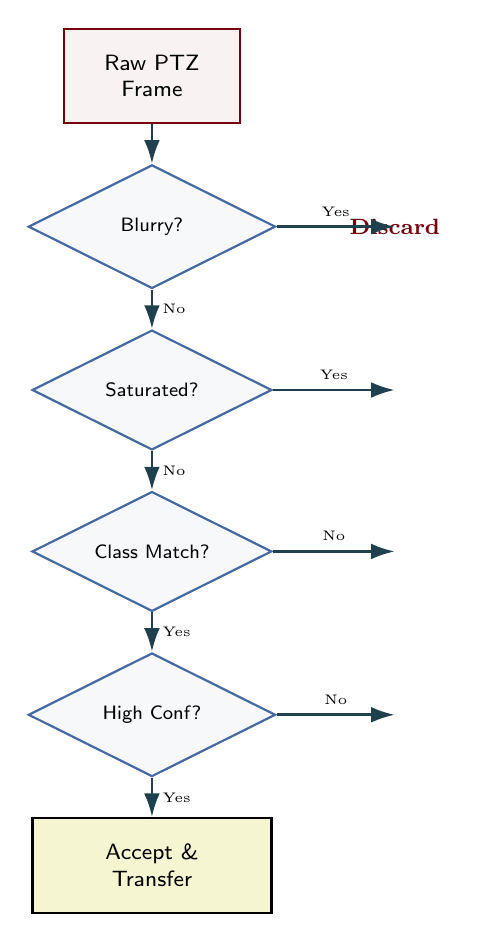
\begin{tikzpicture}[node distance=5mm]
    % Nodes
    \node[data, text width=2cm] (raw) {Raw PTZ\\Frame};

    \node[decision, below=of raw] (blur) {Blurry?};
    \node[decision, below=of blur] (sat) {Saturated?};
    \node[decision, below=of sat] (class) {Class Match?};
    \node[decision, below=of class] (conf) {High Conf?};

    \node[flatblock, below=of conf, fill=CLime!20] (accept) {Accept \&\\Transfer};

    \node[coordinate, right=1.5cm of blur] (discard) {};
    \node[text=Garnet, font=\footnotesize\bfseries] at (discard) {Discard};

    % Paths
    \draw[flatarrow] (raw) -- (blur);

    \draw[flatarrow] (blur.south) -- node[right, font=\tiny] {No} (sat.north);
    \draw[flatarrow] (blur.east) -- node[above, font=\tiny] {Yes} (discard |- blur);

    \draw[flatarrow] (sat.south) -- node[right, font=\tiny] {No} (class.north);
    \draw[flatarrow] (sat.east) -- node[above, font=\tiny] {Yes} (discard |- sat);

    \draw[flatarrow] (class.south) -- node[right, font=\tiny] {Yes} (conf.north);
    \draw[flatarrow] (class.east) -- node[above, font=\tiny] {No} (discard |- class);

    \draw[flatarrow] (conf.south) -- node[right, font=\tiny] {Yes} (accept.north);
    \draw[flatarrow] (conf.east) -- node[above, font=\tiny] {No} (discard |- conf);

\end{tikzpicture}
\caption{Quality Gate Logic. To prevent dataset contamination (drift), PTZ frames must pass a series of deterministic checks for image quality (blur, saturation) and content verification before being used to generate labels.}
\label{fig:gates}
\end{figure}

\subsection{Dataset Schema}
Each committed example stores the wide frame (or short clip), the transferred label, and acquisition metadata. Table~\ref{tab:schema} defines a minimal schema sufficient for training and analysis.

\begin{table}[t]
\centering
\caption{Minimal dataset record schema for each accepted acquisition.}
\label{tab:schema}
\begin{tabular}{@{}ll@{}}
\toprule
Field & Description \\
\midrule
timestamp\_w & Wide-frame timestamp (monotonic) \\
image\_w & Wide image (or video clip key) \\
bbox\_w & Label box in wide coordinates \\
class & Target class (airplane for the test case) \\
score\_w & Wide detector confidence at time $t$ \\
timestamp\_p & PTZ-frame timestamp used for confirmation \\
telemetry\_p & PTZ pan/tilt/zoom, focus, exposure \\
bbox\_p, score\_p & PTZ detector box and confidence \\
quality\_metrics & Blur, saturation, occlusion flags \\
site\_meta & Location, camera orientation, weather \\
\bottomrule
\end{tabular}
\end{table}

\section{Airplanes-in-the-Sky Test Case}
\subsection{Operating Conditions and Target Characteristics}
Airplanes introduce systematic small-object issues. In a wide-angle view, aircraft can be extremely small with strong scale variation as they traverse the sky and change apparent altitude and distance (Fig.~\ref{fig:zoomlevels}). Visual appearance changes with viewing angle, contrails, lighting, haze, and compression artifacts, matching known difficulty factors for small objects (low detail, interference, background ambiguity).
\par
Flying-object detection has been studied with YOLOv8 as a practical real-time architecture choice, and YOLO-family surveys emphasize why these models are frequently deployed in resource-constrained real-time settings.

\begin{figure*}[t]
\centering
\includegraphics[width=1.0\textwidth]{fig_zoom_comparison.pdf}
\caption{Zoom level comparison. At wide-angle (left), a distant airplane may occupy only 15 pixels---insufficient for reliable classification. Progressive zoom increases pixel count, enabling confident detection at 20x zoom (right).}
\label{fig:zoomlevels}
\end{figure*}

\subsection{Class Taxonomy and Negatives}
For this test case, the primary class is \textit{airplane}. Hard negatives arise from birds, insects near the lens, distant drones, clouds with sharp edges, sensor noise, and specular highlights (Fig.~\ref{fig:negatives}). The PTZ confirmation step naturally collects informative negatives: wide proposals that are rejected by PTZ as non-airplane can be stored as hard negatives with contextual metadata.

\begin{figure}[t]
\centering
\includegraphics[width=0.7\columnwidth]{fig_hard_negatives.pdf}
\caption{Hard negative examples. Common false positives in the wide camera include birds, cloud edges, drones, sun glare, insects near the lens, and distant antennas. PTZ verification rejects these as non-airplane.}
\label{fig:negatives}
\end{figure}

\section{Evaluation Protocol}
This paper describes a system design and an evaluation plan intended to be executed on a real deployment. The core evaluation objective is to measure whether PTZ-assisted acquisition yields higher-quality labels and better downstream small-object performance than passive wide-only collection.

\subsection{Baselines}
The following baselines support attribution of improvements to PTZ zoom verification rather than to data volume alone:
\par
A wide-only baseline that logs candidate detections from the wide camera without PTZ confirmation; \par
a PTZ patrol baseline that performs a scripted scan independent of wide detections; \par
a manual-zoom oracle baseline on a small audited subset, used only to estimate upper bounds and error modes.

\subsection{Metrics}
Label quality is assessed on an audited subset using human review or higher-resolution reference footage. Primary metrics include (i) label precision and recall for accepted samples, (ii) bounding-box IoU between transferred labels and audited labels, (iii) confidence uplift $\Delta s = s^p - s^w$ for confirmed samples (Fig.~\ref{fig:uplift}), and (iv) downstream detector performance (e.g., small-object mAP on wide-angle imagery) after training on the constructed dataset.
\par
Because PTZ tracking introduces dynamics and latency, system metrics include slew-to-lock time, dwell time per target, fraction of triggers that successfully reacquire the target, and PTZ availability contention (fraction of time PTZ is busy). PTZ tracking literature suggests these measures are essential to understanding real-world performance beyond static detection accuracy.

\begin{figure}[t]
\centering
\includegraphics[width=0.7\columnwidth]{fig_confidence_uplift.pdf}
\caption{Confidence uplift visualization. Points above the diagonal $s^p = s^w$ indicate samples where PTZ verification increased detection confidence. Low-confidence wide detections (left region) can achieve high PTZ confidence, validating the zoom-based verification approach.}
\label{fig:uplift}
\end{figure}

\subsection{Ablation Factors}
Ablations should isolate contributions from (i) trigger thresholds and hysteresis, (ii) motion prediction vs reactive centering, (iii) zoom scheduling, (iv) label transfer method (direction-only vs depth-aware if depth is available), and (v) pseudo-label admission thresholds. Adaptive pseudo-label thresholding methods provide a useful reference point for designing these ablations.

\section{Implementation Considerations}
\subsection{Real-Time Constraints}
The wide-angle detector must run at frame rate to maintain coverage. YOLO-family models are commonly selected for this regime; Ultralytics documentation notes YOLOv8 release and positioning as a speed--accuracy option for detection tasks, and survey work summarizes the evolution of YOLO variants and real-time deployment considerations.
\par
The PTZ control loop must tolerate latency in (i) wide detection, (ii) command transmission, (iii) mechanical motion, and (iv) PTZ video encoding/decoding. A practical design uses a bounded queue for PTZ commands, drops stale commands, and prioritizes keeping the target near the PTZ image center over maximizing instantaneous zoom.

\subsection{Telemetry Synchronization}
Accurate label transfer requires time alignment between wide frames, PTZ frames, and PTZ telemetry. The system should log monotonic timestamps at capture and at inference, and it should record the PTZ telemetry state at the exact time a PTZ frame is captured (or as close as the interface permits). If telemetry is sampled asynchronously, interpolation to the frame time reduces geometric error.

\subsection{Safety and Privacy}
The airplane test case naturally focuses on sky regions; nonetheless, deployment should constrain PTZ tilt limits and define privacy-preserving regions to avoid capturing ground-level imagery. These constraints can be implemented at the control layer by rejecting commands that enter prohibited zones.

\section{Discussion}
\subsection{When PTZ Verification Helps Most}
PTZ verification is most valuable when the wide detector frequently encounters ambiguous, small candidates whose pixel support is insufficient for confident classification. In such regimes, zoom provides additional evidence without changing the wide camera that will ultimately run the detector. This can be especially beneficial when the deployment environment differs from training data and when pseudo-labeling would otherwise be unreliable.
\par
The approach is aligned with modern PTZ-assisted perception systems that explicitly integrate deep detection with PTZ imaging to improve small-target observability.

\subsection{Limitations}
The system is constrained by single-PTZ availability and cannot zoom multiple targets simultaneously. Fast-moving targets may leave the PTZ field of view during slew, particularly when latency is high or the wide tracker is unstable. Atmospheric turbulence and haze can reduce the effective benefit of zoom. Direction-only label transfer assumes small parallax; large baselines or nearer targets require depth-aware mapping.

\subsection{Extensions}
Multi-PTZ configurations can reduce contention and increase throughput. Joint scheduling across targets can be formulated as a knapsack-like selection over predicted utilities. More advanced multi-view techniques may reduce reliance on explicit calibration in some settings, although the sky-target scenario is favorable for calibration-based geometry due to strong distance scale separation.

\section{Conclusion}
This paper presented a dual-camera active acquisition method for fully automated small-object dataset construction using a fixed wide-angle camera with real-time detection and a PTZ camera for zoom-based verification. For airplanes in the sky, the PTZ view provides higher-resolution evidence that can be transferred back to wide-angle frames to produce higher-quality labels, hard negatives, and metadata. We detailed calibration and control formulations, label transfer procedures, and drift-control gates grounded in pseudo-labeling and PTZ tracking insights from the literature. The proposed evaluation protocol measures label quality, confidence uplift, and downstream small-object performance, enabling rigorous assessment of whether sensor-driven ``auto-labeling'' can replace or substantially reduce manual annotation in small-object regimes.

\begin{thebibliography}{99}

\bibitem{nikouei2024smallobj}
M. Nikouei et al., ``Small Object Detection: A Comprehensive Survey on Challenges, Techniques, and Real-World Applications,'' \textit{Intelligent Systems with Applications}, vol. 25, 2025. doi: \url{10.1016/j.iswa.2025.200561}

\bibitem{mahaur2022superres}
B. Mahaur, N. Singh, and K. K. Mishra, ``Road object detection: a comparative study of deep learning-based algorithms,'' \textit{Multimedia Tools and Applications}, vol. 81, no. 10, pp. 14247-14282, 2022. doi: \url{10.1007/s11042-022-12447-5}

\bibitem{rozantsev2017flying}
A. Rozantsev, V. Lepetit and P. Fua, ``Detecting Flying Objects Using a Single Moving Camera,'' \textit{IEEE Transactions on Pattern Analysis and Machine Intelligence}, vol. 39, no. 5, pp. 879-892, 1 May 2017. doi: \url{10.1109/TPAMI.2016.2564408}

\bibitem{chen2020survey}
G. Chen, H. Pu, W. Luo, and L. Zhang, ``A Survey of the Four Pillars for Small Object Detection: Multiscale Representation, Contextual Information, Super-Resolution, and Region Proposal,'' \textit{IEEE Transactions on Systems, Man, and Cybernetics: Systems}, vol. 52, no. 2, pp. 936-953, Feb. 2022. doi: \url{10.1109/TSMC.2020.3005231}

\bibitem{zhang2019zoom}
X. Zhang, Q. Chen, R. Ng, and V. Koltun, ``Zoom to Learn, Learn to Zoom,'' in \textit{Proceedings of the IEEE/CVF Conference on Computer Vision and Pattern Recognition (CVPR)}, pp. 3762-3770, 2019. doi: \url{10.1109/CVPR.2019.00388}

\bibitem{yolo_flying}
``Real-Time Flying Object Detection with YOLOv8,'' \textit{arXiv preprint arXiv:2305.09972}, 2023. doi: \url{10.48550/arXiv.2305.09972}

\bibitem{ptz_eval}
``Evaluation of trackers for Pan-Tilt-Zoom Scenarios,'' \textit{arXiv preprint arXiv:1711.04260}, 2017. doi: \url{10.48550/arXiv.1711.04260}

\bibitem{ptz_reproducible}
``Reproducible Evaluation of Pan-Tilt-Zoom Tracking,'' in \textit{Proceedings of the IEEE International Conference on Image Processing (ICIP)}, 2015. doi: \url{10.1109/ICIP.2015.7351162}

\bibitem{active_ptz}
``Active Visual Perception Enhancement Method Based on Deep Reinforcement Learning,'' \textit{Electronics}, vol. 13, no. 9, p. 1654, 2024. doi: \url{10.3390/electronics13091654}

\bibitem{anomalous_ptz}
``Anomalous object detection by active search with PTZ cameras,'' \textit{Expert Systems with Applications}, vol. 184, p. 115150, 2021. doi: \url{10.1016/j.eswa.2021.115150}

\bibitem{vigia_ptz}
``VIGIA-E: Density-Aware Patch Selection for Efficient Video Surveillance with PTZ Cameras,'' in \textit{Proceedings of the 25th International Conference on Computer Analysis of Images and Patterns (CAIP)}, 2025. doi: \url{10.1007/978-3-032-04968-1_23}

\bibitem{self_training}
``Adaptive Self-Training for Object Detection,'' in \textit{Proceedings of the IEEE/CVF International Conference on Computer Vision Workshops (ICCVW)}, 2023. doi: \url{10.1109/ICCVW60793.2023.00102}

\bibitem{self_training_enh}
``Improving Object Detection Accuracy with Self-Training Based on Bi-Directional Pseudo Label Recovery,'' \textit{Electronics}, vol. 13, no. 12, p. 2230, 2024. doi: \url{10.3390/electronics13122230}

\bibitem{active_learning_survey}
``Ten Years of Active Learning Techniques and Object Detection: A Comprehensive Survey,'' \textit{Applied Sciences}, vol. 13, no. 10, p. 6181, 2023. doi: \url{10.3390/app13169110}

\bibitem{active_learning_ppod}
``Plug and Play Active Learning for Object Detection,'' in \textit{Proceedings of the IEEE/CVF Conference on Computer Vision and Pattern Recognition (CVPR)}, 2024. doi: \url{10.1109/CVPR52733.2024.01684}

\end{thebibliography}

\end{document}
